\documentclass{standalone}
\usepackage{tikz}
\usetikzlibrary{patterns, positioning}


\begin{document}
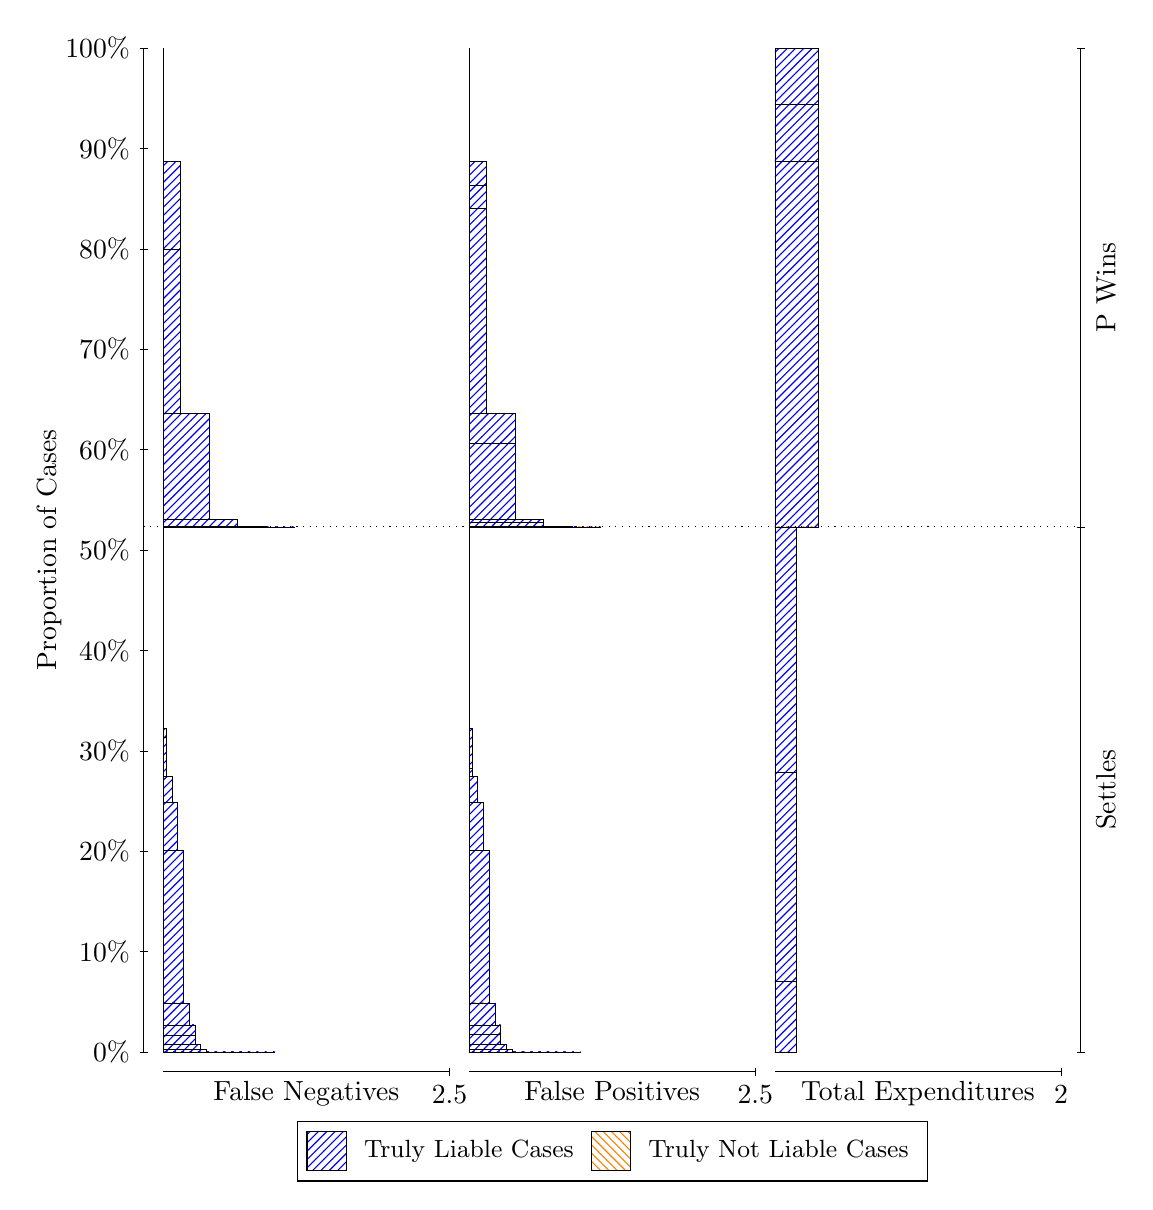
\begin{tikzpicture}
\draw[black, very thin] (1.5,1.75) -- (1.5,14.5);
\node[rotate=90, text=black, anchor=center] at (0.3, 8.125) {Proportion of Cases};
\draw[black, very thin] (1.45,1.75) -- (1.55,1.75);
\node[text=black, anchor=east] at (1.45, 1.75) {0\%};
\draw[black, very thin] (1.45,3.025) -- (1.55,3.025);
\node[text=black, anchor=east] at (1.45, 3.025) {10\%};
\draw[black, very thin] (1.45,4.3) -- (1.55,4.3);
\node[text=black, anchor=east] at (1.45, 4.3) {20\%};
\draw[black, very thin] (1.45,5.575) -- (1.55,5.575);
\node[text=black, anchor=east] at (1.45, 5.575) {30\%};
\draw[black, very thin] (1.45,6.85) -- (1.55,6.85);
\node[text=black, anchor=east] at (1.45, 6.85) {40\%};
\draw[black, very thin] (1.45,8.125) -- (1.55,8.125);
\node[text=black, anchor=east] at (1.45, 8.125) {50\%};
\draw[black, very thin] (1.45,9.4) -- (1.55,9.4);
\node[text=black, anchor=east] at (1.45, 9.4) {60\%};
\draw[black, very thin] (1.45,10.675) -- (1.55,10.675);
\node[text=black, anchor=east] at (1.45, 10.675) {70\%};
\draw[black, very thin] (1.45,11.95) -- (1.55,11.95);
\node[text=black, anchor=east] at (1.45, 11.95) {80\%};
\draw[black, very thin] (1.45,13.225) -- (1.55,13.225);
\node[text=black, anchor=east] at (1.45, 13.225) {90\%};
\draw[black, very thin] (1.45,14.5) -- (1.55,14.5);
\node[text=black, anchor=east] at (1.45, 14.5) {100\%};

\draw[black, very thin] (13.4,1.75) -- (13.4,14.5);
\draw[black, very thin] (13.35,1.75) -- (13.45,1.75);
\node[anchor=west] at (13.35, 1.75) {};
\draw[black, very thin] (13.35,8.4199) -- (13.45,8.4199);
\node[anchor=west] at (13.35, 8.4199) {};
\draw[black, very thin] (13.35,14.5) -- (13.45,14.5);
\node[anchor=west] at (13.35, 14.5) {};

\draw[black, very thin, pattern color=blue, pattern=north east lines] (1.75,1.75) rectangle (3.167,1.75);
\draw[black, very thin, pattern color=blue, pattern=north east lines] (1.75,1.75) rectangle (3.0217,1.75);
\draw[black, very thin, pattern color=blue, pattern=north east lines] (1.75,1.75) rectangle (2.8763,1.75);
\draw[black, very thin, pattern color=blue, pattern=north east lines] (1.75,1.75) rectangle (2.8037,1.75);
\draw[black, very thin, pattern color=blue, pattern=north east lines] (1.75,1.75) rectangle (2.731,1.75);
\draw[black, very thin, pattern color=blue, pattern=north east lines] (1.75,1.75) rectangle (2.6583,1.75);
\draw[black, very thin, pattern color=blue, pattern=north east lines] (1.75,1.75) rectangle (2.5857,1.7501);
\draw[black, very thin, pattern color=blue, pattern=north east lines] (1.75,1.7501) rectangle (2.513,1.7507);
\draw[black, very thin, pattern color=blue, pattern=north east lines] (1.75,1.7507) rectangle (2.4403,1.7523);
\draw[black, very thin, pattern color=blue, pattern=north east lines] (1.75,1.7523) rectangle (2.3677,1.7523);
\draw[black, very thin, pattern color=blue, pattern=north east lines] (1.75,1.7523) rectangle (2.295,1.7839);
\draw[black, very thin, pattern color=blue, pattern=north east lines] (1.75,1.7839) rectangle (2.2223,1.8415);
\draw[black, very thin, pattern color=blue, pattern=north east lines] (1.75,1.8415) rectangle (2.1497,1.9649);
\draw[black, very thin, pattern color=blue, pattern=north east lines] (1.75,1.9649) rectangle (2.1497,2.095);
\draw[black, very thin, pattern color=blue, pattern=north east lines] (1.75,2.095) rectangle (2.077,2.3732);
\draw[black, very thin, pattern color=blue, pattern=north east lines] (1.75,2.3732) rectangle (2.0043,2.3734);
\draw[black, very thin, pattern color=blue, pattern=north east lines] (1.75,2.3734) rectangle (2.0043,4.3118);
\draw[black, very thin, pattern color=blue, pattern=north east lines] (1.75,4.3118) rectangle (1.9317,4.9244);
\draw[black, very thin, pattern color=blue, pattern=north east lines] (1.75,4.9244) rectangle (1.859,5.2454);
\draw[black, very thin, pattern color=blue, pattern=north east lines] (1.75,5.2454) rectangle (1.7863,5.7452);
\draw[black, very thin, pattern color=blue, pattern=north east lines] (1.75,5.7452) rectangle (1.7863,5.858);
\draw[black, very thin, pattern color=orange, pattern=north west lines] (1.75,5.858) rectangle (1.75,5.858);
\draw[black, very thin, pattern color=blue, pattern=north east lines] (1.75,5.858) rectangle (1.75,8.4199);
\draw[black, very thin, pattern color=blue, pattern=north east lines] (1.75,8.4199) rectangle (3.4213,8.4199);
\draw[black, very thin, pattern color=blue, pattern=north east lines] (1.75,8.4199) rectangle (3.058,8.4208);
\draw[black, very thin, pattern color=blue, pattern=north east lines] (1.75,8.4208) rectangle (2.6947,8.515);
\draw[black, very thin, pattern color=blue, pattern=north east lines] (1.75,8.515) rectangle (2.3313,9.8608);
\draw[black, very thin, pattern color=blue, pattern=north east lines] (1.75,9.8608) rectangle (1.968,11.95);
\draw[black, very thin, pattern color=blue, pattern=north east lines] (1.75,11.95) rectangle (1.968,13.059);
\draw[black, very thin, pattern color=orange, pattern=north west lines] (1.75,13.059) rectangle (1.75,13.059);
\draw[black, very thin, pattern color=blue, pattern=north east lines] (1.75,13.059) rectangle (1.75,14.5);
\draw[black, very thin, pattern color=orange, pattern=north west lines] (5.6333,1.75) rectangle (7.0503,1.75);
\draw[black, very thin, pattern color=blue, pattern=north east lines] (5.6333,1.75) rectangle (7.0503,1.75);
\draw[black, very thin, pattern color=orange, pattern=north west lines] (5.6333,1.75) rectangle (6.905,1.75);
\draw[black, very thin, pattern color=blue, pattern=north east lines] (5.6333,1.75) rectangle (6.905,1.75);
\draw[black, very thin, pattern color=orange, pattern=north west lines] (5.6333,1.75) rectangle (6.7597,1.75);
\draw[black, very thin, pattern color=blue, pattern=north east lines] (5.6333,1.75) rectangle (6.7597,1.75);
\draw[black, very thin, pattern color=blue, pattern=north east lines] (5.6333,1.75) rectangle (6.687,1.75);
\draw[black, very thin, pattern color=orange, pattern=north west lines] (5.6333,1.75) rectangle (6.6143,1.75);
\draw[black, very thin, pattern color=blue, pattern=north east lines] (5.6333,1.75) rectangle (6.6143,1.75);
\draw[black, very thin, pattern color=blue, pattern=north east lines] (5.6333,1.75) rectangle (6.5417,1.75);
\draw[black, very thin, pattern color=orange, pattern=north west lines] (5.6333,1.75) rectangle (6.469,1.75);
\draw[black, very thin, pattern color=blue, pattern=north east lines] (5.6333,1.75) rectangle (6.469,1.7501);
\draw[black, very thin, pattern color=blue, pattern=north east lines] (5.6333,1.7501) rectangle (6.3963,1.7507);
\draw[black, very thin, pattern color=orange, pattern=north west lines] (5.6333,1.7507) rectangle (6.3237,1.7507);
\draw[black, very thin, pattern color=blue, pattern=north east lines] (5.6333,1.7507) rectangle (6.3237,1.7523);
\draw[black, very thin, pattern color=blue, pattern=north east lines] (5.6333,1.7523) rectangle (6.251,1.7523);
\draw[black, very thin, pattern color=orange, pattern=north west lines] (5.6333,1.7523) rectangle (6.1783,1.7523);
\draw[black, very thin, pattern color=blue, pattern=north east lines] (5.6333,1.7523) rectangle (6.1783,1.7839);
\draw[black, very thin, pattern color=blue, pattern=north east lines] (5.6333,1.7839) rectangle (6.1057,1.8415);
\draw[black, very thin, pattern color=orange, pattern=north west lines] (5.6333,1.8415) rectangle (6.033,1.8415);
\draw[black, very thin, pattern color=blue, pattern=north east lines] (5.6333,1.8415) rectangle (6.033,1.9716);
\draw[black, very thin, pattern color=blue, pattern=north east lines] (5.6333,1.9716) rectangle (6.033,2.095);
\draw[black, very thin, pattern color=blue, pattern=north east lines] (5.6333,2.095) rectangle (5.9603,2.3732);
\draw[black, very thin, pattern color=orange, pattern=north west lines] (5.6333,2.3732) rectangle (5.8877,2.3732);
\draw[black, very thin, pattern color=blue, pattern=north east lines] (5.6333,2.3732) rectangle (5.8877,4.3117);
\draw[black, very thin, pattern color=blue, pattern=north east lines] (5.6333,4.3117) rectangle (5.8877,4.3119);
\draw[black, very thin, pattern color=blue, pattern=north east lines] (5.6333,4.3119) rectangle (5.815,4.9245);
\draw[black, very thin, pattern color=blue, pattern=north east lines] (5.6333,4.9245) rectangle (5.7423,5.2454);
\draw[black, very thin, pattern color=blue, pattern=north east lines] (5.6333,5.2454) rectangle (5.6697,5.3581);
\draw[black, very thin, pattern color=blue, pattern=north east lines] (5.6333,5.3581) rectangle (5.6697,5.858);
\draw[black, very thin, pattern color=blue, pattern=north east lines] (5.6333,5.858) rectangle (5.6333,8.4199);
\draw[black, very thin, pattern color=orange, pattern=north west lines] (5.6333,8.4199) rectangle (7.3047,8.4199);
\draw[black, very thin, pattern color=blue, pattern=north east lines] (5.6333,8.4199) rectangle (7.3047,8.4199);
\draw[black, very thin, pattern color=orange, pattern=north west lines] (5.6333,8.4199) rectangle (6.9413,8.4199);
\draw[black, very thin, pattern color=blue, pattern=north east lines] (5.6333,8.4199) rectangle (6.9413,8.4201);
\draw[black, very thin, pattern color=blue, pattern=north east lines] (5.6333,8.4201) rectangle (6.9413,8.4208);
\draw[black, very thin, pattern color=orange, pattern=north west lines] (5.6333,8.4208) rectangle (6.578,8.4208);
\draw[black, very thin, pattern color=blue, pattern=north east lines] (5.6333,8.4208) rectangle (6.578,8.4709);
\draw[black, very thin, pattern color=blue, pattern=north east lines] (5.6333,8.4709) rectangle (6.578,8.515);
\draw[black, very thin, pattern color=orange, pattern=north west lines] (5.6333,8.515) rectangle (6.2147,8.515);
\draw[black, very thin, pattern color=blue, pattern=north east lines] (5.6333,8.515) rectangle (6.2147,9.4844);
\draw[black, very thin, pattern color=blue, pattern=north east lines] (5.6333,9.4844) rectangle (6.2147,9.8608);
\draw[black, very thin, pattern color=blue, pattern=north east lines] (5.6333,9.8608) rectangle (5.8513,12.462);
\draw[black, very thin, pattern color=orange, pattern=north west lines] (5.6333,12.462) rectangle (5.8513,12.462);
\draw[black, very thin, pattern color=blue, pattern=north east lines] (5.6333,12.462) rectangle (5.8513,12.761);
\draw[black, very thin, pattern color=blue, pattern=north east lines] (5.6333,12.761) rectangle (5.8513,13.059);
\draw[black, very thin, pattern color=blue, pattern=north east lines] (5.6333,13.059) rectangle (5.6333,14.5);
\draw[black, very thin, pattern color=orange, pattern=north west lines] (9.5167,1.75) rectangle (9.7892,1.75);
\draw[black, very thin, pattern color=blue, pattern=north east lines] (9.5167,1.75) rectangle (9.7892,2.6486);
\draw[black, very thin, pattern color=orange, pattern=north west lines] (9.5167,2.6486) rectangle (9.7892,2.6486);
\draw[black, very thin, pattern color=blue, pattern=north east lines] (9.5167,2.6486) rectangle (9.7892,5.3031);
\draw[black, very thin, pattern color=orange, pattern=north west lines] (9.5167,5.3031) rectangle (9.7892,5.3031);
\draw[black, very thin, pattern color=blue, pattern=north east lines] (9.5167,5.3031) rectangle (9.7892,8.4199);
\draw[black, very thin, pattern color=orange, pattern=north west lines] (9.5167,8.4199) rectangle (10.062,8.4199);
\draw[black, very thin, pattern color=blue, pattern=north east lines] (9.5167,8.4199) rectangle (10.062,13.061);
\draw[black, very thin, pattern color=orange, pattern=north west lines] (9.5167,13.061) rectangle (10.062,13.061);
\draw[black, very thin, pattern color=blue, pattern=north east lines] (9.5167,13.061) rectangle (10.062,13.78);
\draw[black, very thin, pattern color=orange, pattern=north west lines] (9.5167,13.78) rectangle (10.062,13.78);
\draw[black, very thin, pattern color=blue, pattern=north east lines] (9.5167,13.78) rectangle (10.062,14.5);
\draw[black, dotted] (1.5,8.4199) -- (13.4,8.4199);
\draw[black, very thin] (1.75,1.5) -- (5.3833,1.5);
\node[text=black, anchor=north] at (3.5667, 1.5) {False Negatives};
\draw[black, very thin] (5.3833,1.45) -- (5.3833,1.55);
\node[text=black, anchor=north] at (5.3833, 1.45) {2.5};

\draw[black, very thin] (5.6333,1.5) -- (9.2667,1.5);
\node[text=black, anchor=north] at (7.45, 1.5) {False Positives};
\draw[black, very thin] (9.2667,1.45) -- (9.2667,1.55);
\node[text=black, anchor=north] at (9.2667, 1.45) {2.5};

\draw[black, very thin] (9.5167,1.5) -- (13.15,1.5);
\node[text=black, anchor=north] at (11.333, 1.5) {Total Expenditures};
\draw[black, very thin] (13.15,1.45) -- (13.15,1.55);
\node[text=black, anchor=north] at (13.15, 1.45) {2};

\node[text=black, centered, rotate=90] at (13.72, 5.0849) {Settles};
\node[text=black, centered, rotate=90] at (13.72, 11.46) {P Wins};

\draw (7.449999999999999,1.5) node[draw=none] (baseCoordinate) {};
\begin{scope}[align=center]
        \matrix[scale=0.5, draw=black, below=0.5cm of baseCoordinate, nodes={draw}, column sep=0.1cm]{
            \node[rectangle, draw, minimum width=0.5cm, minimum height=0.5cm, pattern color=blue, pattern=north east lines] {}; &
            \node[draw=none, font=\small, text=black] (B) {Truly Liable Cases}; &
            \node[rectangle, draw, minimum width=0.5cm, minimum height=0.5cm, pattern color=orange, pattern=north west lines] {}; &
            \node[draw=none, font=\small, text=black] (B) {Truly Not Liable Cases}; \\
            };
\end{scope}

\end{tikzpicture}
\end{document}